\section{Implementierung in Python}

Nachdem in Kapitel \ref{sec:Auswahl} evaluiert wurde welcher Algorithmus für unsere Problematik am besten angewendet werden kann wurde die Implementierung des \glqq Bees Algorithms\grqq{} in der Programmiersprache Python programmiert.\\\\
Zu Beginn des Programmes musste die Karte mit den dazugehörigen Hindernissen initialisiert werden. Die Karte wurde in Form eines 2D-Koordinatensystems umgesetzt (siehe Abbildung \ref{fig:map_init}).
\begin{figure}[H]
    \begin{tabular}{@{}r@{}} 
        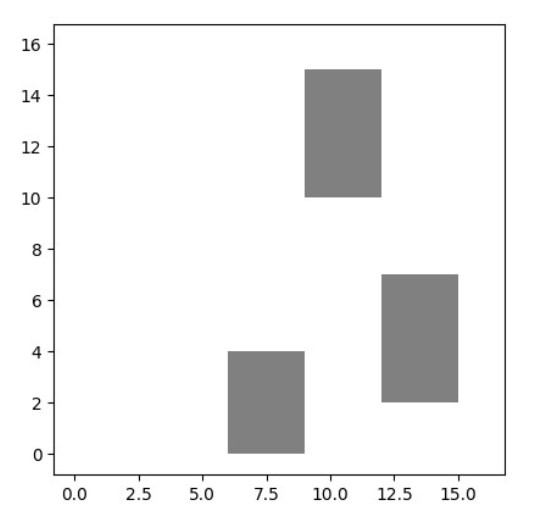
\includegraphics[width=0.5\textwidth, height=0.31\textheight, center]{map_init.jpg}
    \end{tabular}
    \caption{Initialisierte Karte mit Hindernissen\\}   
    \label{fig:map_init}
\end{figure}
Die Menge in der sich der Roboter bewegen darf ergibt sich aus der Gesamtzahl der Karte \emph{K} und den Hindernissen innerhalb der Karte \emph{H}:
\[K\_frei = K - H\]
Als nächstes wird, wie bereits in Kapitel \ref{chap:algorithmen} beschrieben, die Population initialisiert. Für unseren Fall wird der Bienen Algorithmus nicht verwendet um einen optimalen Punkt zu finden, sogar um den optimalen Pfad zu finden. Dabei bildet jede Biene einen Pfad ab. Die Pfade bestehen aus \emph{k} vielen Punkten in Form eines Tuples \emph{(x,y)}. Jeder Pfad wird mit den Koordinaten \emph{(0,0)} initialisiert und muss am Ende am Ziel \emph{(16,16)} ankommen. Die Funktion iteriert von \emph{i = 1} bis \emph{k}, da der erste Punkt des Pfades bereits gesetzt ist:
\begin{figure}[H]
    \begin{lstlisting}[language=python]
def init_population():
    k=7
    i = 1
    path = [(0,0)]
    goal = (16,16)
 while i <= k:
    x = int(random.uniform(0, map_width))
    y = int(random.uniform(0, map_height))
    position = (x,y)
    if is_feasible(position, path[i-1],obstacle_list=obstacle_list):
        path.append((x,y))
        i+=1
    else: 
        x = int(random.uniform(0, map_width))
        y = int(random.uniform(0, map_height))
        position = (x,y)
            
 # Wirf Pfad weg falls das Ziel nach 10 Schritten nicht erreicht ist.
 count = 0
 while not is_feasible(goal,path[i-1],obstacle_list=obstacle_list):
    count += 1
    x = int(random.uniform(0, map_width))
    y = int(random.uniform(0, map_height))
    if is_feasible((x,y), path[i-2], obstacle_list=obstacle_list):
        path[i-1] = (x,y)
    if count > 10:
        return initPopulation()   
    
 path.append(goal)
 return  path
\end{lstlisting}
\caption{init\_population Funktion}
\label{fig:init}
\end{figure} 
Im Quellcode der Abbildung \ref{fig:init} benutzt die stetige Gleichverteilung oder auch uniform distribution function genannt. Die Gleichverteilungsfunktion ist eine Wahrscheinlichkeitsverteilungsfunktion, die angibt, wie wahrscheinlich es ist, dass eine Zufallsvariable einen bestimmten Wert innerhalb eines bestimmten Intervalls annimmt.
Die Gleichverteilungsfunktion ordnet jedem Wert innerhalb des Intervalls die gleiche Wahrscheinlichkeit zu. Das bedeutet, dass jede Zahl innerhalb des Intervalls mit gleicher Wahrscheinlichkeit gezogen wird.\\
Die Formel für die Stetige Gleichverteilung lautet:
\[f(x) = 1/(b-a),\: a \leq x \leq b\]
\[f(x) = 0,\:x < a \:oder\: x > b\]
Dabei ist \emph{a} der untere und \emph{b} der obere Endpunkt des Intervalls \cite{casella2021statistical}. Im Falle dieser Bienen Algorithmus Implementierung wird die Stetige Gleichverteilungsfunktion verwendet, um zufällige Pfadpunkte in den Grenzen der Karte zu erstellen.\\
Nach der Erstellung der Punkte muss überprüft werden, ob der Punkt valide ist. Ein Punkt innerhalb eines Pfades \emph{P} wird als valide angesehen, wenn die folgenden Bedingungen erfüllt sind \cite{Darwish2018}:

\[1. \quad P \cap H = \emptyset \quad\]
\[2. \quad \forall i, \forall j \quad \overline{p_i p_j} \cap H = \emptyset\]

Aus diesen zwei Formeln kann man ableiten, dass in einem validem Pfad weder ein Punkt innerhalb eines Hindernisses liegen darf, noch darf eine Verbindung von zwei Punkten der Menge P ein Hindernis aus der Menge \emph{H} schneiden darf.
Die zwei dazugehörigen Funktion sehen wie folgt aus:


\begin{figure}[H]
    \centering
        \begin{lstlisting}[language=python]
def pointInsideObstacle(point, obstacle):
    # Überprüfen, ob der Punkt innerhalb des Hindernisses liegt
    for obs in obstacle:
        if point[0] == obs[0] and point[1] == obs[1]:
            return True
                
    return False
            \end{lstlisting}
    \caption{Überprüfen ob der Punkt in einem Hindernis liegt}
      \label{fig:pointInsideObstacle}
\end{figure}

\begin{figure}[H]
    \begin{lstlisting}[language=python]
def intersects(point1, point2, obstacle):
 # Überprüfen, ob die Strecke von point1 zu point2 das Hindernis schneidet

 x_min = min(point1[0], point2[0])
 x_max = max(point1[0], point2[0])
 y_min = min(point1[1], point2[1])
 y_max = max(point1[1], point2[1])

 for obs in obstacle:
    if obs[0] >= x_min and obs[0] <= x_max and obs[1] >= y_min and obs[1] <= y_max:
        return True
return False
    \end{lstlisting}
    \caption{Überprüfen ob Schnittpunkt existiert}
\end{figure}

Aus diesen zwei Funktion setzt sich die Funktion \emph{is\_feasible()} zusammen, die in der Methode \emph{init\_population()} verwendet wird. Ein neuer Punkt wird also nur hinzugefügt, falls \emph{is\_feasible} wahr ist. Eine Ausnahme die existiert entsteht bei dem Anfügen des letzten Punktes \emph{(16,16)}. Es kann passieren, dass der letzte generierte Punkt des Pfades keine valide Verbindung zu dem Zielpunkt herstellen kann, da immer ein Hindernis im Weg ist. In diesem Falle wird der letzte Punkt des Pfades wieder ersetzt durch einen neuen Punkt. Im Anschluss wird überprüft, ob dieser Punkt nun auf gültigem Wege zum Ziel kommt. Falls dies nach 10 Versuchen nicht funktioniert wird der Pfad komplett wegeworfen und neu initialisiert. Diese Variante stellte sich nach vermehrten Überprüfungen als effizientesten Weg heraus.\\

Für die weiteren Schritte des Bienen Algorithmus benötigen wir die Bewertungsfunktion. Die Bewertung eines Pfades wird mithilfe des Euklidischen Abstands berechnet:
\[f = \sum_{i=1}^{n-1} \sqrt{(x_{i+1} - x_i)^2 + (y_{i+1} - y_i)^2}\]\newpage Der Euklidische Abstand berechnet den Abstand zwischen zwei Punkten innerhalb einer Ebene \cite{Friedrich2019}. Dies wird für jeden Punkt durchgeführt und aufsummiert. Die passende Funktion dazu sieht wie folgt aus:

\begin{figure}[H]
    \begin{lstlisting}[language=python]
def evaluate_path(path):
    x_points = []
    y_points= []
    for i in range(len(path)):
        x, y = path[i]
        x_points.append(x)
        y_points.append(y)
    i=1
    total_distance= 0
    while i < len(path)-1:
        total_distance += np.sqrt((x_points[i+1] - x_points[i]) **2 + (y_points[i+1] - y_points[i])**2)
        i+=1
        return total_distance
    \end{lstlisting}
    \caption{Evaluierungsfunktion}
\end{figure}

In Kombination mit der Evaluierungsfunktion wird die Lokale Suche des Bienen Algorithmus angewandt, um in einer bestimmten Umgebung, auch Nachbarschaft genannt, zu suchen. Dafür kann die Größe der Nachbarschaft \emph{ngh} beliebig initialisiert werden. Nachfolgend wird für jeden Punkt des Pfades der übergeben wird, außer für Start und Ziel, ein neuer Punkt mittels Stetiger Gleichverteilungsfunktion in einer bestimmten Begrenzung erstellt. Dabei muss allerdings sichergestellt werden, dass ein valider Punkt dem Pfad hinzugefügt wird. Falls der Punkt ungültig ist wird ein neuer Punkt erstellt. Zum Schluss der Funktion wird überprüft ob die Fitness des neuen Pfades höher ist als die des alten Pfades. Wenn das der Fall ist wird der Pfad akualisiert. Auf diese Weise versucht man die bestehenden Pfade zu optimieren.   

\begin{figure}[H]
    \begin{lstlisting}[language=python]
def local_search(solution, fitness):
    ngh = 2
    i = 1
    while i <= len(solution) - 2:
     count= 0
     new_solution = solution.copy()
     new_point =  (int(random.uniform(solution[i][0]-ngh, solution[i][0]+ngh)),int(random.uniform(solution[i][1]-ngh, solution[i][1]+ngh)))
     new_solution[i] = new_point
     while not path_is_feasible(new_solution):
        new_point =  (int(random.uniform(solution[i][0]-ngh, solution[i][0]+ngh)),int(random.uniform(solution[i][1]-ngh, solution[i][1]+ngh)))
         new_solution[i] = new_point 
         count +=1
         if count > 20:
            return solution
        new_fitness = evaluate_path(new_solution)
        if new_fitness < fitness:
            solution = new_solution
        i+= 1
    return solution
    \end{lstlisting}
    \caption{Lokale Suche des Bienen Algorithmus}
\end{figure}

Neben der lokalen Suche findet eine globale Suche statt. Hier werden erneut randomisiert eine Menge an Pfaden erstellt und per Evaluationsfunktion bewertet. Dieses Mal wird allerdings nicht die stetige Gleichverteilungsfunktion verwendet, sondern wählt man eine zufällige Stelle im Pfad aus und generiert dort eine zufällige Änderung bewirkt. Diese neu-erstellten Pfade wird im Anschluss zurückgegeben und zur Gesamtmenge der gefunden Pfade hinzugefügt.

\begin{figure}[H]
    \begin{lstlisting}[language=python]
def generate_new_solutions(solutions, best_solution):
    new_solutions = []
    for solution in solutions:
        # Wenn die Lösung mit der besten Lösung übereinstimmt, wird sie übersprungen
        if solution == best_solution:
            continue
        
        # Zufällige Stelle im Pfad auswählen
        index = random.randint(1, len(solution)-2)
        
        # Neue Lösung generieren durch zufällige Änderung an der ausgewählten Stelle
        new_solution = solution.copy()
        new_x = new_solution[index][0] 
        new_y = new_solution[index][1] 
        new_solution[index] = (new_x, new_y)
        
        # Neue Lösung zur Lösungsmenge hinzufügen
        new_solutions.append(new_solution)
    
    return new_solutions
    \end{lstlisting}
    \caption{Globale Suche des Bienen Algorithmus}
\end{figure}

Zuletzt müssen diese Methoden auf die Weise, wie in Kaptitel \ref{chap:algorithmen} erläutert wurde, in einer Funktion zusammengefügt werden. Diese Funktion nimmt als Parameter die Anzahl an Kundschafter Bienen, die auch als Anzahl der Iterationen gesehen werden kann, und sieht wie folgt aus:
\begin{figure}[H]
    \begin{lstlisting}[language=python]
def bees_algorithm(num_scouts):
 i=0
 solutions = []
 while i <= num_scouts:    
    path = initPopulation()
    solutions.append(path)
        i+=1

 for i in range(num_scouts):
 # Führe Local Search für jede Lösung durch
    for j in range(len(solutions)):
        solutions[j] = local_search(solutions[j], evaluate_path(solutions[j]))

    # Berechne Fitness-Werte der Lösungen
    fitnesses = [evaluate_path(solution) for solution in solutions]

    # Aktualisiere die beste Lösung (findet niedrigsten Wert im Array)
    best_solution_index = np.argmin(fitnesses)
    best_solution = solutions[best_solution_index]

    # Generiere neue Lösungen durch globale Suche
    new_solutions = generate_new_solutions(solutions, best_solution)

    # Sortiere Array aufsteigend
    fitnesses = sorted(fitnesses)

    # Aktualisiere die Lösungsmenge mit den neuen Lösungen
    solutions[num_scouts:] = new_solutions

 return solutions, best_solution
\end{lstlisting}
\caption{Gesamtheit des Bienen Algorithmus}
\end{figure}
Zu Beginn des Algorithmus wird die Population initialisiert auf die Anzahl der Kundschafter Bienen. Anschließend wird für jeden Pfad die lokale Suche durchgeführt, die Fitness berechnet und die beste Lösung aktualisiert. Zudem wird die Globale Suche angewandt und das Array aufsteigend anhand der Fitness-Werte sortiert. Die neu-generierten Fitness-Werte werden nun an den Index der Anzahl von Kundschafter Bienen des Arrays angehängt, damit die Menge der Pfade nicht zu groß wird und somit die Funktion effizienter ist.  
In dieser Implementierung wurde als Stoppkriterium die Menge an Iterationen gewählt, jedoch lässt sich dieses beliebig wählen. Ein weiteres sinnvolles Stoppkriterium wäre beispielsweise ein bestimmter Fitness-Wert. \\\\
Nach 30 Iterationen hat der Bienen Algorithmus den folgenden Pfad errechnet:
\begin{figure}[H]
    \begin{tabular}{@{}r@{}} 
        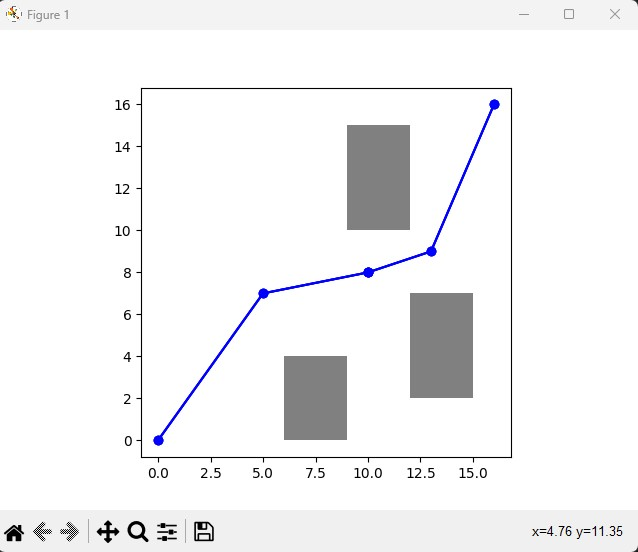
\includegraphics[width=0.5\textwidth, height=0.31\textheight, center]{schnellster_weg.jpg}
    \end{tabular}
    \caption{Schnellster Pfad mit 30 Iterationen\\}   
    \label{fig:schnellster}
\end{figure}

Zur Veranschaulichung, welche Wege der Bienen Algorithmus verwendet hat, wurde die Gesamtheit aller Pfade graphisch dargestellt:
\begin{figure}[H]
    \begin{tabular}{@{}r@{}} 
        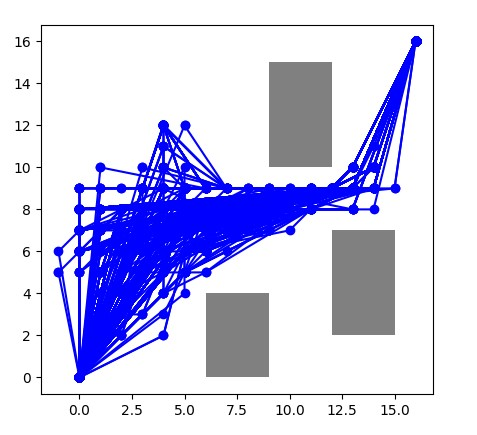
\includegraphics[width=0.5\textwidth, height=0.31\textheight, center]{passende_iterationen.jpg}
    \end{tabular}
    \caption{Initialisierte Karte mit Hindernissen\\}   
    \label{fig:iterationen}
\end{figure}

In Abbildung \ref{fig:iteration} ist die funktionsweise des Bienen Algorithmus zu erkennen. Verschiedene Punkte mittels der Lokalen Suche wurden ausgetestet, um den bestmöglichen Weg zu finden.